
\subsection{RQ4: Which Short-Burst GPU Tracing Policies Work Best?}
\label{sec:rq4}

\subsubsection{Evaluation Approach}

RQ4 compares the six stopping policies via offline replay over real L4 vLLM window evidence, avoiding additional expensive Nsight executions per policy. Each policy is replayed over the same per-window evidence streams, so differences in outcome are attributable solely to the stopping condition rather than to workload variation or profiler noise. This assumes a policy's stopping choice does not meaningfully change later windows' evidence; we expect this confound to be small since T0/T1 collection is always-on and policy-independent, and RQ3 bounds the profiler's own T0/T1 perturbation at under 1\%.

We use two replay datasets. The \emph{stable replay} uses the real automatic-mode windows from the six vLLM serving scenarios across three seeds (18 streams). In this dataset the correct bottleneck label appears in the first suspicious window for every stream, making it an easy diagnostic setting. The \emph{ambiguity stress replay} uses the same 18 streams with the first suspicious window in each stream relabeled as unknown, modeling the realistic case where a single burst is insufficient. The stress dataset is the primary discriminating evaluation because it separates policies that can handle ambiguous early windows from those
that cannot.

\subsubsection{Metrics}

We report mean top-1 accuracy, premature-stop rate, re-escalation-needed rate (the fraction of streams with suspicious windows remaining after the policy stops), mean heavy-trace duration, and duration saved relative to the Repeated Fixed Burst baseline ($N=3$). These are combined into a composite score weighted 40\% accuracy, 25\% premature-stop avoidance, 20\% re-escalation avoidance, and 15\% cost-efficiency.\footnote{Composite score $= 0.40 \times \text{accuracy} + 0.25 \times (1 - \text{premature-stop rate}) + 0.20 \times (1 - \text{re-escalation rate}) + 0.15 \times \text{cost-efficiency}$, where cost-efficiency is the normalised inverse of mean trace duration.}

\subsubsection{Stable Replay Results}

The stable replay is not the discriminating condition --- every policy reaches top-1 accuracy of 1.0 with zero premature stops --- so its results are summarized in text rather than a table. \textsc{CR} and \textsc{HS} avoided re-escalation entirely but required 34.9\,s of tracing per episode, whereas \textsc{FB} used 10.0\,s but left suspicious windows after stopping. \textsc{MU} and \textsc{SS} were Pareto-dominated by \textsc{FB}: they incurred twice the tracing cost (20.0\,s) without improving accuracy or re-escalation rate. \textsc{RFB} fell between these extremes (30.0\,s, re-escalation rate 0.8) and remained Pareto-efficient only because no other policy matched its particular cost--reliability point.

\subsubsection{Ambiguity Stress Replay Results}

Table~\ref{tab:rq4-stress} reports policy rankings on the ambiguity stress dataset, which
is the primary discriminating evaluation.

\begin{table*}[t]
\centering
\caption{RQ4 ambiguity stress policy ranking (18 streams, first window relabeled as
unknown). \textsc{FB} fails entirely; multi-window policies recover to top-1 accuracy
of 1.0.}
\label{tab:rq4-stress}
\footnotesize
\setlength{\tabcolsep}{4pt}
\renewcommand{\arraystretch}{0.95}
\begin{tabular}{clrrrrrrl}
\toprule
\textbf{Rank} & \textbf{Policy} & \textbf{Top-1} & \textbf{Premature} &
\textbf{Re-esc.} & \textbf{Trace (s)} & \textbf{Saved (\%)} &
\textbf{Score} & \textbf{Pareto} \\
\midrule
1 & \textsc{CR} & 1.0 & 0.0 & 0.0 & 34.9 & $-16.3$ & 0.868 & yes \\
2 & \textsc{HS} & 1.0 & 0.0 & 0.0 & 34.9 & $-16.3$ & 0.868 & yes \\
3 & \textsc{MU} & 1.0 & 0.0 & 0.8 & 30.0 &    0.0  & 0.720 & yes \\
4 & \textsc{RFB} & 1.0 & 0.0 & 0.8 & 30.0 &   0.0  & 0.720 & yes \\
5 & \textsc{SS} & 1.0 & 0.0 & 0.8 & 30.0 &    0.0  & 0.720 & yes \\
6 & \textsc{FB} & 0.0 & 1.0 & 1.0 & 10.0 & $+66.7$ & 0.112 & yes \\
\bottomrule
\end{tabular}
\end{table*}

The stress dataset clearly separates one-burst and multi-burst policies.
\textsc{FB} fails completely: its top-1 accuracy drops to 0.0 and its premature-stop rate
rises to 1.0, because it commits to the ambiguous first-window unknown label and never
collects the additional burst needed to reach the concrete diagnosis.
Despite this failure, \textsc{FB} still shows Pareto-efficient in Table~\ref{tab:rq4-stress}, since no policy beats it on cost alone; Pareto status must therefore be read alongside accuracy and premature-stop rate, not as a standalone selection criterion.

All five multi-window policies recover to a top-1 accuracy of 1.0 and a premature-stop
rate of 0.0.
\textsc{CR} and \textsc{HS} again rank highest with a re-escalation rate of 0.0,
confirming their robustness as safety-first policies: they wait for both diagnosis
stability and workload recovery before stopping, ensuring no suspicious windows remain.

\textsc{MU}, \textsc{SS}, and \textsc{RFB} are tied at rank 3--5 with a re-escalation
rate of 0.83 and a mean trace duration of 30\,s. \textsc{MU} and \textsc{SS} are
preferable to \textsc{RFB} since they stop on evidence convergence rather than a
fixed burst count.

\subsubsection{Policy Tradeoff Analysis}

Figure~\ref{fig:rq4-tradeoff} illustrates the cost--safety tradeoff across the six
policies on the stress dataset.

\begin{figure}[t]
\centering
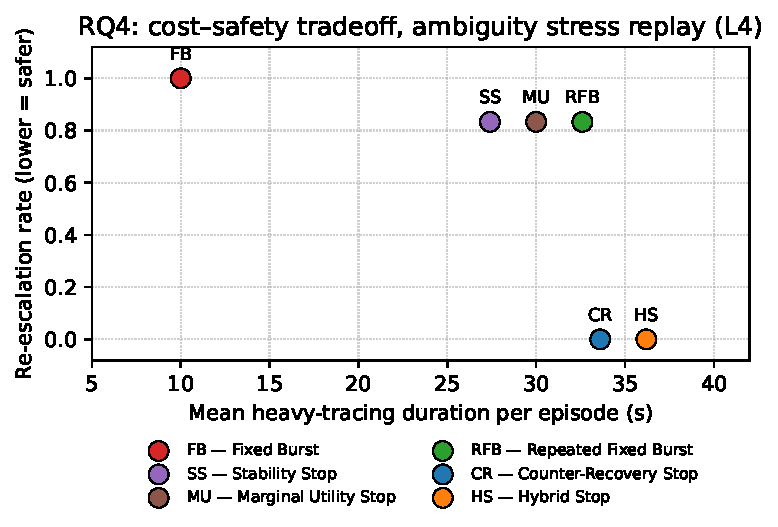
\includegraphics[width=\columnwidth]{figures/rq4_tradeoff.pdf}
\caption{Cost--safety tradeoff across the six stopping policies on the ambiguity stress dataset (Table~\ref{tab:rq4-stress}). \textsc{CR} and \textsc{HS} achieve zero re-escalation at higher trace cost; \textsc{MU}, \textsc{RFB}, and \textsc{SS} trade a 0.8 re-escalation rate for lower cost; \textsc{FB} is cheapest but fails outright (top-1 accuracy 0.0) rather than merely re-escalating.}
\label{fig:rq4-tradeoff}
\end{figure}

\subsubsection{RQ4: Answer}

No single policy dominates all dimensions, so the right choice depends on operator priorities. For safety-first deployments, \textsc{Hybrid Stop} and \textsc{Counter-Recovery Stop} eliminate re-escalation entirely and are robust to ambiguous first windows, at the cost of about 16\% more trace budget than \textsc{RFB}. For budget-aware deployments, \textsc{Stability Stop} and \textsc{Marginal Utility Stop} achieve 1.0 top-1 accuracy with 33\% less trace time than the recovery-gated policies, accepting a re-escalation rate of approximately 0.83. \textsc{Fixed Burst} is not robust as a standalone policy: it fails completely when the first profiler window is ambiguous, with a top-1 accuracy of 0.0 and a premature-stop rate of 1.0 on the stress dataset.